\documentclass[a4paper]{article}
\usepackage[T1]{fontenc}
\usepackage[russian]{babel}
\usepackage[pdftex]{graphicx}
\usepackage[ruled,vlined]{algorithm2e}
\usepackage[utf8]{inputenc}
\usepackage{xcolor}
\usepackage{hyperref}
\usepackage{amsmath}
\usepackage{geometry}
\usepackage{float}
\usepackage{caption}
\usepackage{subcaption}
\DeclareGraphicsExtensions{.pdf,.png,.jpg}

\begin{document}

    \begin{titlepage}
        \Large
        \begin{center}
            Санкт-Петербургский \ Политехнический университет Петра Великого\\
            \vspace{10em}Отчет по лабораторной работе №3\\
            \vspace{2em}
            \textbf{Анализ выбросов в распределениях}
        \end{center}
        \vspace{6em}
        \hfill\parbox{10cm}{
            \hspace*{2cm}\hspace*{-4cm}Студент:\hfill Швачко Никита Андреевич\\
            \hspace*{2cm}\hspace*{-4cm}Преподаватель:\hfill Баженов Александр Николаевич\\
            \hspace*{2cm}\hspace*{-4cm}Группа:\hfill 5030102/20202
        }
        \vspace{\fill}
        \begin{center}
            Санкт-Петербург \ 2025
        \end{center}
    \end{titlepage}


    \section{Формулировка задания и его формализация}\label{sec:task}
    Для анализа двухмерных нормальных распределений и смесей нормальных распределений необходимо:
    \begin{enumerate}
        \item Сгенерировать выборки размерами 20, 60 и 100 элементов для нормального двумерного распределения $N(x, y, 0,0,1,1,\rho)$ с коэффициентами корреляции $\rho = 0.0, 0.5, 0.9$.
        \item Каждая выборка генерируется 1000 раз, после чего вычисляются следующие статистики:
        \begin{itemize}
            \item Среднее значение для коэффициентов корреляции Пирсона, Спирмена и квадрантного коэффициента корреляции.
            \item Среднее значение квадрата этих коэффициентов.
            \item Дисперсия этих коэффициентов.
        \end{itemize}
        \item Повторить все вычисления для смеси нормальных распределений:
        $$f(x, y) = 0.9 N(x, y, 0,0,1,1,0.9) + 0.1 N(x, y, 0,0,10,10,-0.9)$$
        \item Изобразить сгенерированные точки на плоскости и нарисовать эллипс равновероятности для каждого случая.
    \end{enumerate}


    \section{Сгенерированные точки и эллипсы равновероятности}\label{sec:scatterplots}
    Для каждой выборки была выполнена генерация точек и построение эллипсов равновероятности. Ниже представлены графики сгенерированных точек для различных коэффициентов корреляции.

    \begin{figure}[H]
        \centering
        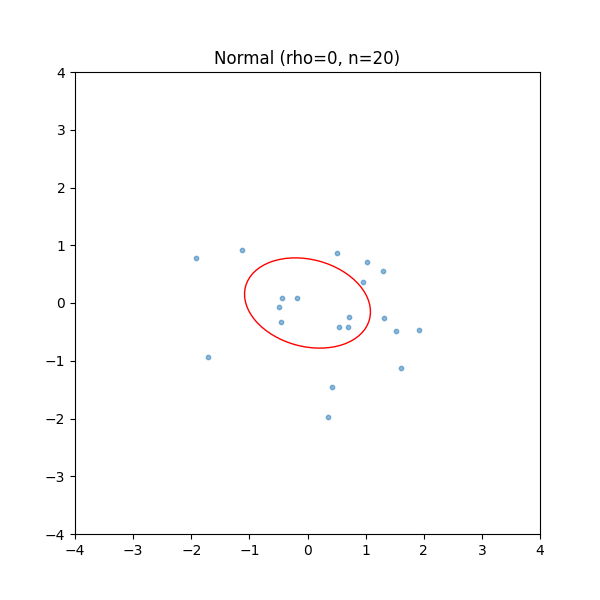
\includegraphics[width=0.8\textwidth]{./plots/normal_rho0_n20}
        \caption{Генерация точек для $\rho = 0.0$ и эллипс равновероятности для $n=20$}
        \label{fig:normal_rho0_n20}
    \end{figure}

    \begin{figure}[H]
        \centering
        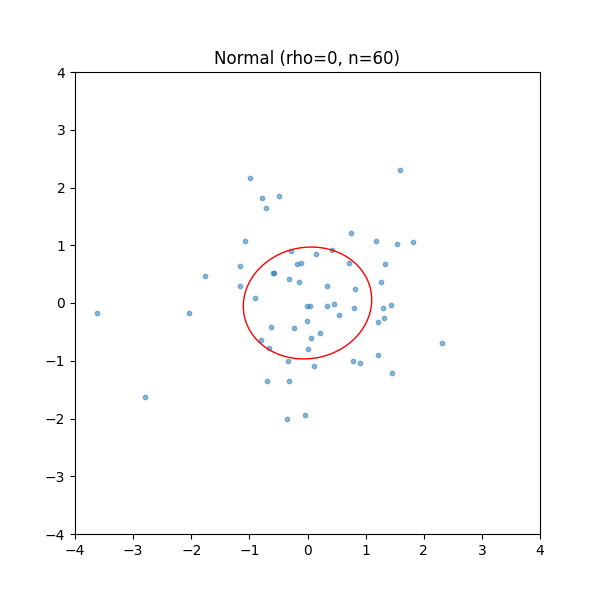
\includegraphics[width=0.8\textwidth]{./plots/normal_rho0_n60}
        \caption{Генерация точек для $\rho = 0.0$ и эллипс равновероятности для $n=60$}
        \label{fig:normal_rho0_n60}
    \end{figure}

    \begin{figure}[H]
        \centering
        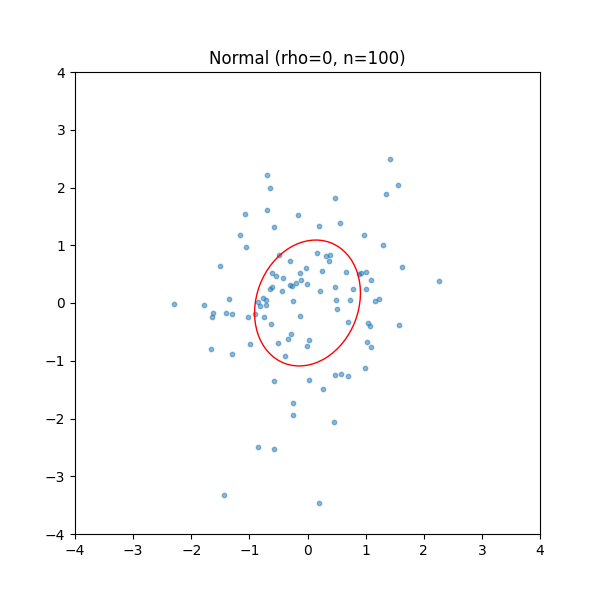
\includegraphics[width=0.8\textwidth]{./plots/normal_rho0_n100}
        \caption{Генерация точек для $\rho = 0.0$ и эллипс равновероятности для $n=100$}
        \label{fig:normal_rho0_n100}
    \end{figure}

    \begin{figure}[H]
        \centering
        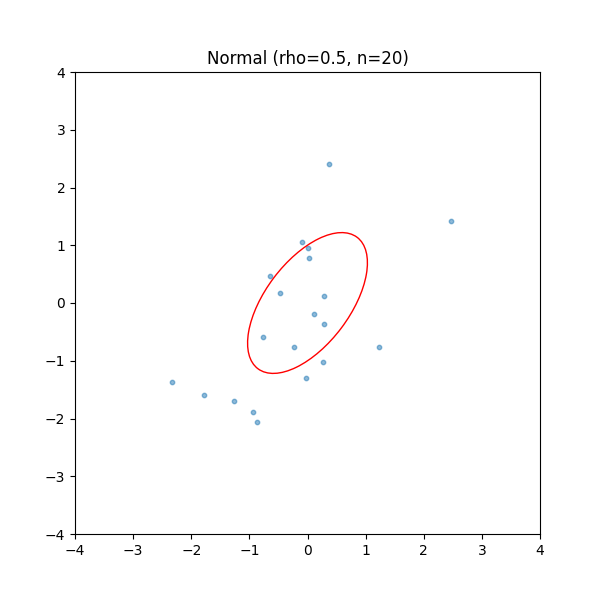
\includegraphics[width=0.8\textwidth]{./plots/normal_rho0.5_n20}
        \caption{Генерация точек для $\rho = 0.5$ и эллипс равновероятности для $n=20$}
        \label{fig:normal_rho0.5_n20}
    \end{figure}

    \begin{figure}[H]
        \centering
        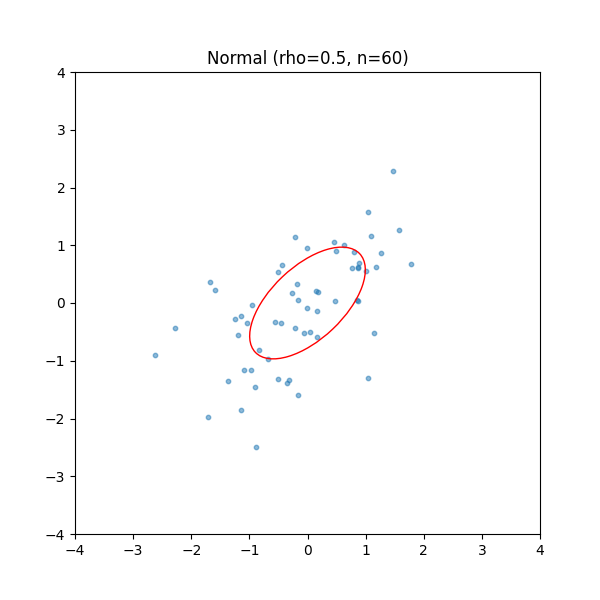
\includegraphics[width=0.8\textwidth]{./plots/normal_rho0.5_n60}
        \caption{Генерация точек для $\rho = 0.5$ и эллипс равновероятности для $n=60$}
        \label{fig:normal_rho0.5_n60}
    \end{figure}

    \begin{figure}[H]
        \centering
        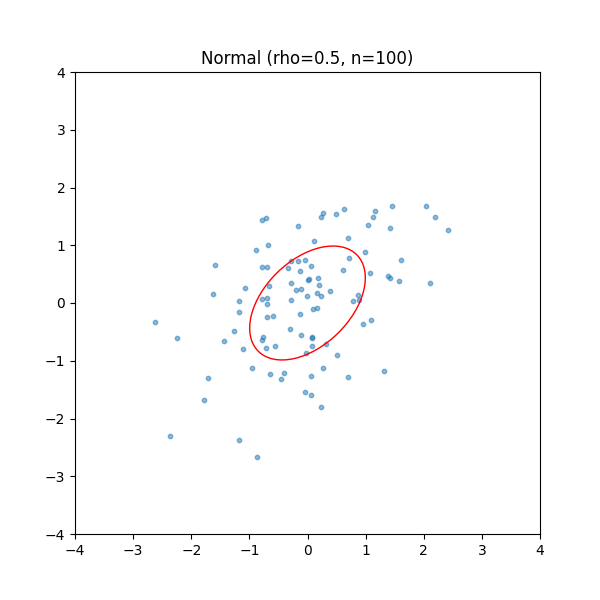
\includegraphics[width=0.8\textwidth]{./plots/normal_rho0.5_n100}
        \caption{Генерация точек для $\rho = 0.5$ и эллипс равновероятности для $n=100$}
        \label{fig:normal_rho0.5_n100}
    \end{figure}

    \begin{figure}[H]
        \centering
        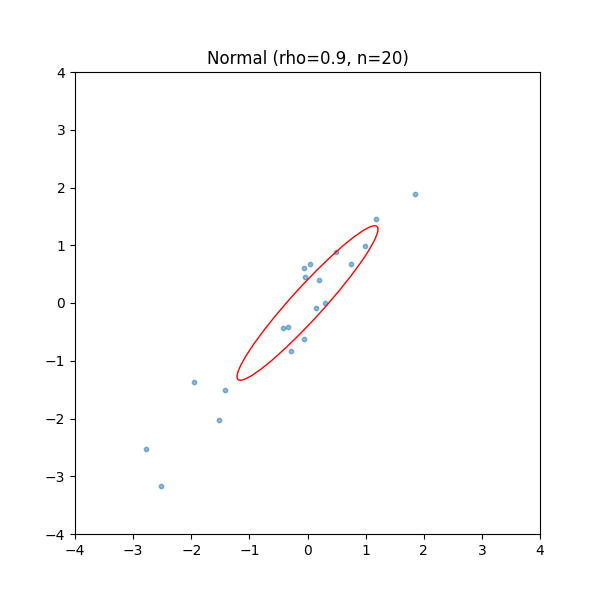
\includegraphics[width=0.8\textwidth]{./plots/normal_rho0.9_n20}
        \caption{Генерация точек для $\rho = 0.9$ и эллипс равновероятности для $n=20$}
        \label{fig:normal_rho0.9_n20}
    \end{figure}

    \begin{figure}[H]
        \centering
        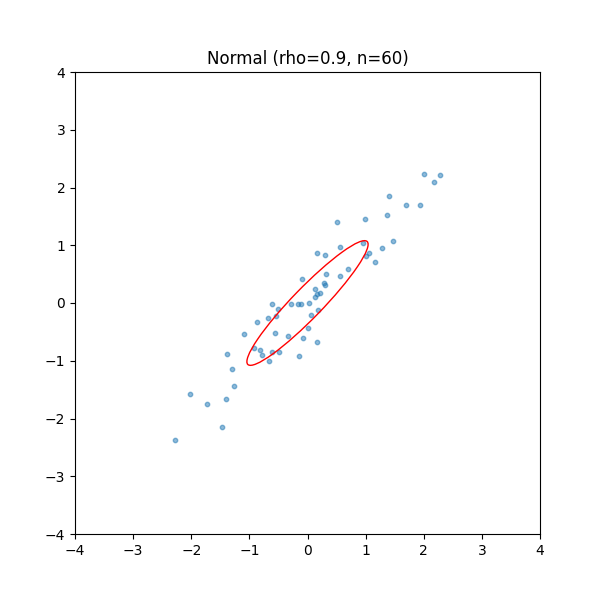
\includegraphics[width=0.8\textwidth]{./plots/normal_rho0.9_n60}
        \caption{Генерация точек для $\rho = 0.9$ и эллипс равновероятности для $n=60$}
        \label{fig:normal_rho0.9_n60}
    \end{figure}

    \begin{figure}[H]
        \centering
        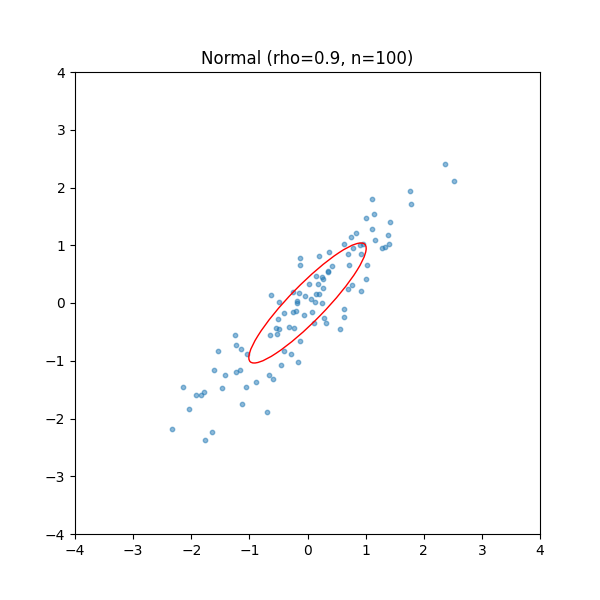
\includegraphics[width=0.8\textwidth]{./plots/normal_rho0.9_n100}
        \caption{Генерация точек для $\rho = 0.9$ и эллипс равновероятности для $n=100$}
        \label{fig:normal_rho0.9_n100}
    \end{figure}


    \section{Результаты для смеси нормальных распределений}\label{sec:mixture_results}
    Также были выполнены вычисления для смеси нормальных распределений. Графики точек и эллипсов равновероятности для смеси представлены ниже.

    \begin{figure}[H]
        \centering
        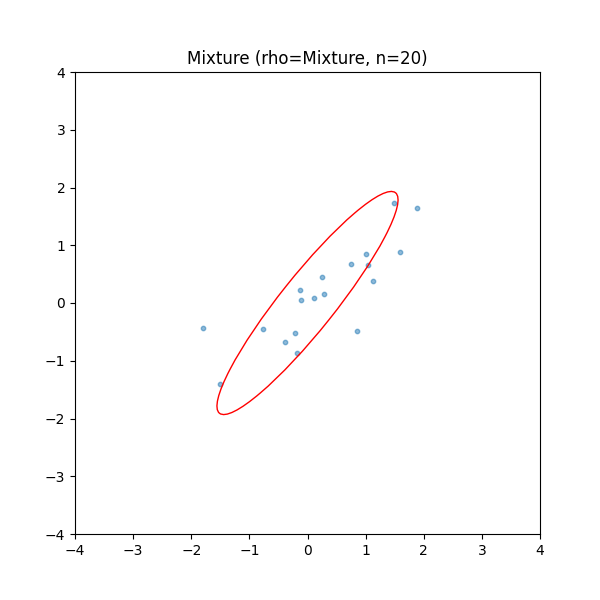
\includegraphics[width=0.8\textwidth]{./plots/mixture_rhoMixture_n20}
        \caption{Генерация точек для смеси с эллипсом равновероятности для $n=20$}
        \label{fig:mixture_rhoMixture_n20}
    \end{figure}

    \begin{figure}[H]
        \centering
        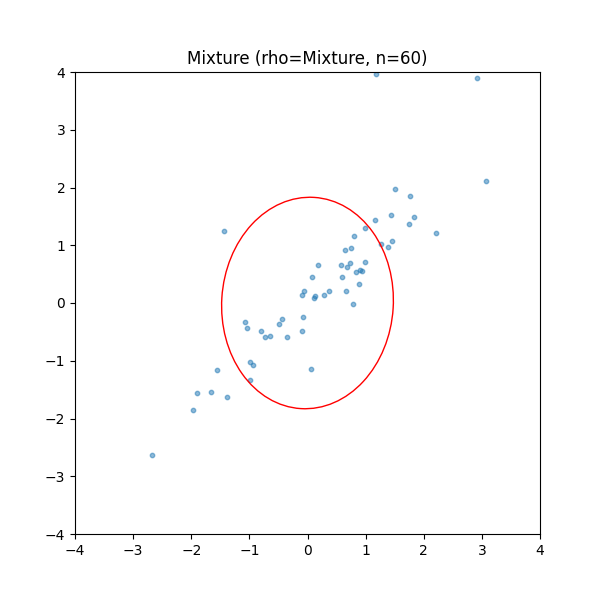
\includegraphics[width=0.8\textwidth]{./plots/mixture_rhoMixture_n60}
        \caption{Генерация точек для смеси с эллипсом равновероятности для $n=60$}
        \label{fig:mixture_rhoMixture_n60}
    \end{figure}

    \begin{figure}[H]
        \centering
        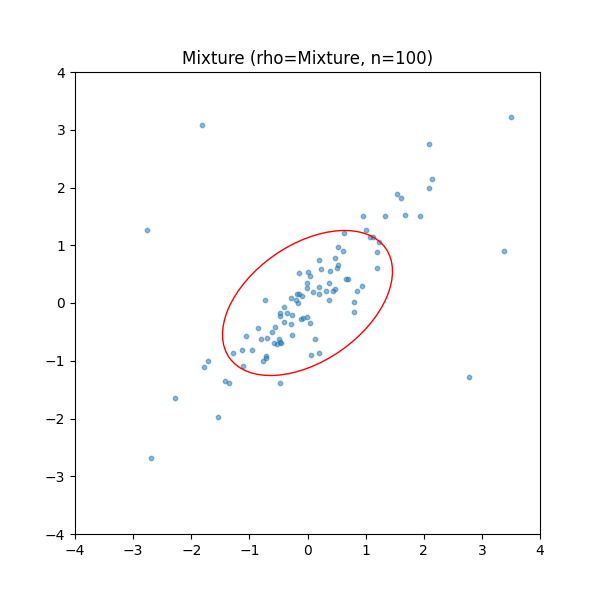
\includegraphics[width=0.8\textwidth]{./plots/mixture_rhoMixture_n100}
        \caption{Генерация точек для смеси с эллипсом равновероятности для $n=100$}
        \label{fig:mixture_rhoMixture_n100}
    \end{figure}


    \section{Результаты вычислений для коэффициентов корреляции}\label{sec:correlation_results}
    В результате вычислений для каждого коэффициента корреляции были получены следующие статистики (среднее значение, среднее квадрата и дисперсия) для выборок размером 20, 60 и 100.
    \begin{table}[!htbp]
        \centering
        \caption{Средние значения и дисперсии коэффициентов корреляции для различных выборок}
        \scalebox{0.8}{
            \begin{tabular*}{\textwidth}{@{\extracolsep{\fill}}|c|c|c|c|}
                \hline
                \textbf{Размер выборки} & \textbf{Коэффициент Пирсона} & \textbf{Коэффициент Спирмена} & \textbf{Квадрантный коэффициент} \\
                \hline
                ('Normal', 0, 20)       & 0.12343                      & 0.05969                       & -0.09170 \\
                ('Normal', 0, 60)       & 0.07463                      & 0.11577                       & 0.19617 \\
                ('Normal', 0, 100)      & 0.14622                      & 0.13461                       & 0.08948 \\
                ('Normal', 0.5, 20)     & 0.56445                      & 0.57348                       & 0.30410 \\
                ('Normal', 0.5, 60)     & 0.40189                      & 0.44387                       & 0.29707 \\
                ('Normal', 0.5, 100)    & 0.44021                      & 0.40305                       & 0.21928 \\
                ('Normal', 0.9, 20)     & 0.95226                      & 0.92174                       & 0.70520 \\
                ('Normal', 0.9, 60)     & 0.93982                      & 0.92567                       & 0.79920 \\
                ('Normal', 0.9, 100)    & 0.90720                      & 0.89664                       & 0.84114 \\
                ('Mixture', '', 20)     & 0.89881                      & 0.83134                       & 0.69410 \\
                ('Mixture', '', 60)     & 0.50792                      & 0.70468                       & 0.53360 \\
                ('Mixture', '', 100)    & 0.51057                      & 0.71010                       & 0.65790                          \\
                \hline
            \end{tabular*}
        }
        \label{tab:correlation_results}

    \end{table}


    \section{Выводы}\label{sec:conclusions}
    \begin{itemize}
        \item Коэффициент корреляции Пирсона, Спирмена и квадрантный коэффициент дают схожие результаты для нормального распределения с высоким коэффициентом корреляции.
        \item Для смеси нормальных распределений результаты отличаются из-за смешанных компонент с различной корреляцией.
        \item Графики и эллипсы равновероятности демонстрируют изменение зависимости между переменными в зависимости от значения коэффициента корреляции.
    \end{itemize}

\end{document}